\documentclass[11pt,a4paper,twocolumn]{article}
\usepackage{geometry}
\usepackage{amsmath}
\usepackage{float}
\usepackage{graphicx}
\usepackage{caption}
\usepackage{subcaption}
\usepackage{hyperref}
\usepackage[T1]{fontenc}
\usepackage[toc,page]{appendix}

\geometry{
	includeheadfoot,
	margin=2.54cm
}

\graphicspath{{img/}}

\catcode`\^^I=13
\catcode`\^^M=13

\newcounter{linenumber}

\newenvironment{sourcecode}{\begingroup%
\setcounter{linenumber}{0}%
\def\algorithm##1{\setcounter{linenumber}{0}\medskip \textbf{Algorithm} \textsc{##1} \parskip=0pt\everypar={\parskip=0pt\stepcounter{linenumber}\rlap{\scriptsize{\thelinenumber}}\qquad}}%
\def\event##1{\setcounter{linenumber}{0}\medskip \textbf{##1:} \parskip=0pt\everypar={\parskip=0pt\stepcounter{linenumber}\rlap{\scriptsize{\thelinenumber}}\qquad}}%
%
\def\comment##1{\textit{//##1}}%
\def\qif##1{\textbf{if} ##1}%
\def\qifdefined##1{\textbf{if} ##1 \textbf{defined}}%
\def\qifndefined##1{\textbf{if} ##1 \textbf{not defined}}%
\def\qelse{\textbf{else}}%
\def\qelseif##1{\textbf{else if ##1}}%
\def\for##1{\textbf{for} ##1}%
\def\foreach##1{\textbf{for each} ##1}%
\def\qdo{\textbf{do}}%
\def\while##1{\textbf{while} ##1}%
\def\return##1{\textbf{return} ##1}%
\def\break{\textbf{break}}%
\def\qglobal##1{\textbf{global} ##1}%
\def\qsend##1{\textbf{send} \emph{##1}}%
\def\qreceive##1{\textbf{receive} \emph{##1}}%
\def\qbegin{\textbf{begin}}
\def\qend{\everypar={}\textbf{end}}
\def\runningtime##1{\hfill ##1}
\catcode`\^^I=13%
\catcode`\^^M=13%
\def^^I{\qquad}%
\def^^M{\par}%
}{\endgroup}

\catcode`\^^I=10
\catcode`\^^M=5


\newfloat{algo}{thp}{lop}
\floatname{algo}{Algorithm}

\title{
	{\huge Project\\ \emph{Parameter-based Island Terrain Generation}}\\
	{\large For 2IV06 - Visual Computing Project}
}
\author{
	T.M. van Dalen \\
	C.J.P. van Dueren den Hollander\\
	{\texttt\{t.m.v.dalen,c.j.p.v.dueren.den.hollander\}}@student.tue.nl
}
\date{\today}

\begin{document}
	\maketitle
	
	\begin{abstract}
	
\end{abstract}

	
	\section{Introduction}
	\label{sec:intro}
	%introduction/requirements
We want to develop a terrain generation algorithm and corresponding viewer. 

Our main inspiration for this project is the article by Patel\cite{redblob}.
The author presents an algorithm for generating terrain maps for games based on certain game design decisions.
Figure~\ref{fig:map-2d} gives an example of a terrain map that was generated by the demonstration implementation of the algorithm.

\begin{figure}[h]
	\centering
	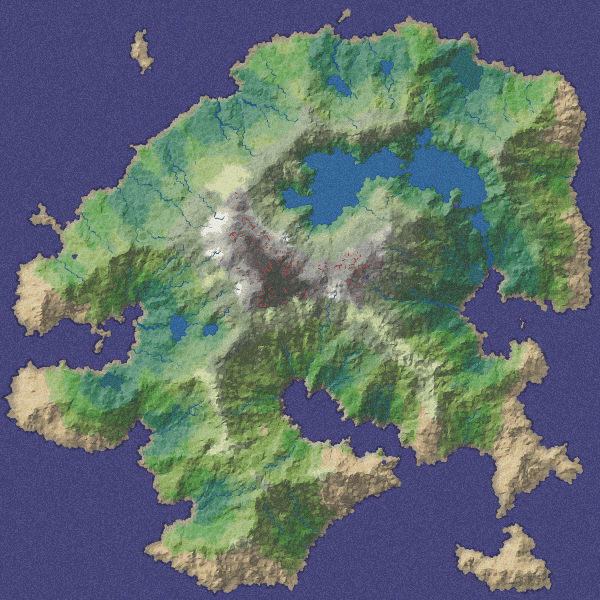
\includegraphics[width=\linewidth]{map-2d}
	\caption{An example terrain}
	\label{fig:map-2d}
\end{figure}

While we do not intend to follow the same general rules for terrain generation, the author gives a clear description of the algorithm which we should be able to use to develop an algorithm for our specific use case.
Most importantly, the goal in the paper is to generate a mountainous island that gets higher the further one goes inland.
While this is not a bad approximation of reality, we feel it is too strong, and that it results in terrains that are not easily explored 'on foot'.

The author makes some interesting suggestions for future work.

Our most important requirement for the terrain viewer is that it should be able to easily explore the generated terrain.
We will at least implement a mode for 'walking', but we may add more feature if this enables easier exploration.

Furthermore, we want to explore the possibility of adding NPC's that can move through the generated world, similar to Braitenberg vehicles.
Their path will be influenced by biomes or affected by obstructions such as rivers and mountains.
A certain NPC might prefer dry biomes and be unable to scale mountainous terrain or one might be able to cross water and be constrained to stay in moist biomes.

Since the goal of the terrain generator is to create a natural terrain, we would like for the terrain viewer to also visualise the terrain in a life-like way.
This includes using textures for different biomes and animating bodies of water.

The terrain generation algorithm is the focus of our project.

The author of \cite{redblob} does not give any way to explore the terrain.
The demonstration implementation does however have a few different terrain viewers, among which is a 3D viewer, shown in Figure~\ref{fig:map-3d}.
We do not want to implement these simple viewers, though they might be useful for debugging.

\begin{figure}[h]
	\centering
	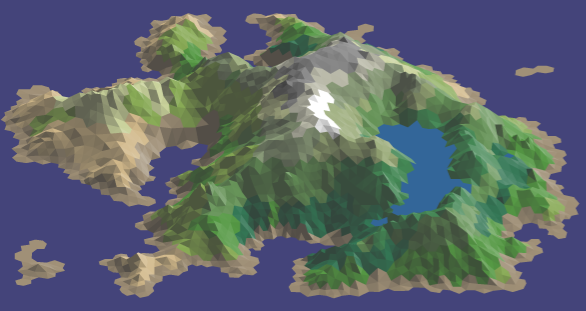
\includegraphics[width=\linewidth]{map-3d}
	\caption{A 3D render of the map depicted in Figure~\ref{fig:map-2d}}
	\label{fig:map-3d}
\end{figure}

	
	\section{Analysis}
	\label{sec:analysis}
	%analysis and solution: mathematics/algorithms/system design

\subsection{Data structures}

We call the final generated terrain a \textbf{Map}.
A Map is a collection of \textbf{Center}s, \textbf{Corner}s and \textbf{Edge}s.

\paragraph{Center} has the following properties:

\begin{itemize}
	\item Vec2 point
	\item bool water
	\item bool ocean
	\item bool coast
	\item bool border
	\item float elevation
	\item float moisture
	\item Biome biome
	\item Center[] neighbours
	\item Edge[] borders
	\item Corner[] corners
\end{itemize}

\paragraph{Corner} has the following properties:

\begin{itemize}
	\item Vec2 point
	\item bool water
	\item bool ocean
	\item bool coast
	\item bool border
	\item float elevation
	\item float moisture
	\item int river
	\item int watershed\_size
	\item Corner downslope
	\item Corner watershed
	\item Center[] touches
	\item Edge[] protrudes
	\item Corner[] adjacent
\end{itemize}

\paragraph{Edge} has the following properties:

\begin{itemize}
	\item Center delaunay0
	\item Center delaunay1
	\item Corner voronoi0
	\item Corner voronoi1
	\item int river
	\item Vec2 midway\_point
\end{itemize}

\subsection{Generation}

The terrain generation happens in the following stages:

\begin{enumerate}
	\item Placing points
	\item Building graph
	\item Shaping island
	\item Assigning elevations
	\item Assigning moisture and rivers
	\item Assigning biomes
\end{enumerate}

\paragraph{Placing points}

In this stage, the points that make up the center of the polygons are selected.
We currently have a selector that returns random points, one that uses poisson trials for better randomness, one that returns points that result in a hexagonal voronoi diagram and one that results in a grid-like voronoi diagram.

The selected points become the centers of the map.

Figure~\ref{fig:algo:points} shows an example of selected points.

Algorithm~\ref{alg:point} gives pseudo-code for the point selector that results in a grid-like structure.

\begin{algo*}
\begin{sourcecode}
\algorithm{SquarePointSelector($width, height, n$)}
$P = \emptyset$
\for{$i = 0; i < \sqrt{n}; i++$}
	\for{$i = 0; i < \sqrt{n}; i++$}
		$P = P \cup \left<\frac{0.5 + i}{n} width, \frac{0.5 + j}{n} height\right>$
	|
|
\return P
\qend
\end{sourcecode}
	\caption{Point selection}
	\label{alg:point}
\end{algo*}

\paragraph{Building graph}

Next, we use the selected points to build the data structures that represent the map.
We do this by constructing a Voronoi diagram (using Fortune's algorithm) and a Delaunay triangulation and creating polygons from that.

All nodes in the Voronoi diagram become corners, all edges in the Voronoi diagram, together with their dual edge in the Delaunay triangulation, are saved as edges in the map.

Pseudo-code for this can be found in Algorithm~\ref{alg:graph}

Figure~\ref{fig:algo:voronoi} shows an example of a generated Voronoi diagram, Figure~\ref{fig:algo:delaunay} gives the resulting Delaunay triangulation.

\begin{algo*}
\begin{sourcecode}
\algorithm{BuildGraph($P$)}
$V, D =$ \textsc{GenerateVoronoi}($P$)
$centers = $\textsc{MakeCenters}($P$)
\for{$e \in V,D$}
	$edge = $\{
		\textsc{GetCenter}($centers, e.delaunay0$),
		\textsc{GetCenter}($centers, e.delaunay1$),
		\textsc{MakeCorner}($e.voronoi0$),
		\textsc{MakeCorner}($e.voronoi1$)
	\}
	\textsc{SetupRelations}($edge$)
|
\return centers
\qend
\end{sourcecode}
	\caption{Graph building}
	\label{alg:graph}
\end{algo*}

\paragraph{Shaping island}

The island shape is a function that determines which of the centers in the map are part of the island and which are water.

In Figure~\ref{fig:algo:polygons}, an example island shape is shown.

Algorithm~\ref{alg:shape} gives an example of a map shaper that results in a round island.

\begin{algo*}
\begin{sourcecode}
\algorithm{RoundMapShaper($p$)}
\return $p.x^2 + p.y^2 < 1$
\qend
\end{sourcecode}
	\caption{Shaping the island}
	\label{alg:shape}
\end{algo*}

\paragraph{Assigning elevations}

In the elevations step, we first assign elevations to corners by going from the ocean inwards, increasing the elevation by 1 whenever we move to a new rank.
Then, we redistribute the elevations by sorting all corners on elevation, and evenly distributing elevations from 0 to 1 among them.
Finally, we set the elevation of each center to the average of its corners.

Figure~\ref{fig:algo:elevation} gives an example of elevations.

Algorithm~\ref{alg:elevation} gives an overview of the elevation assignment.
Pseudo-code for its components will follow.

\begin{algo*}
\begin{sourcecode}
\algorithm{AssignElevations($shaper$)}
\textsc{AssignElevationsCorner}($shaper$)
\textsc{AssignElevationsCoastAndLand}()
\textsc{AssignElevationsRedistribute}()
\textsc{AssignElevationsPolygons}()
\qend
\end{sourcecode}
	\caption{Elevation overview}
	\label{alg:elevation}
\end{algo*}

\paragraph{Assigning moisture and rivers}

First, we calculate the corner that is downslope for each corner in the map.
Then, we use this to calculate watersheds.
After that, we randomly select a number of springs on the map, where we start a river.
From each spring, we follow the watershed corners until we reach the ocean.

Then, we assign moisture to each corner based on the distance to a river or a body of water and we redistribute moisture like elevation.
Finally, we set the moisture of each center to the average of its corners.

Algorithm~\ref{alg:moisture} gives an overview of the moisture assignment.
Pseudo-code for its components will follow.

\begin{algo*}
\begin{sourcecode}
\algorithm{AssignMoisture()}
\textsc{calculateDownslopes}()
\textsc{calculateWatersheds}()
\textsc{createRivers}()
\textsc{assignCornerMoisture}()
\textsc{assignMoistureRedistribute}()
\textsc{assignPolygonMoisture}()
\qend
\end{sourcecode}
	\caption{Moisture overview}
	\label{alg:moisture}
\end{algo*}

\paragraph{Assigning biomes}

Finally, we use the moisture and elevation properties of each center to assign a biome.

Algorithm~\ref{alg:biome} gives an impression of how this could happen, the real implementation is much more detailed.

\begin{algo*}
\begin{sourcecode}
\algorithm{getBiome($center$)}
\qif{$center.ocean$}
	\return \texttt{OCEAN}
\qelse
	\qif{$center.moisture > 0.7$}
		\return \texttt{SWAMP}
	\qelse
		\qif{$center.elevation < 0.5$}
			\return \texttt{PLAINS}
		\qelse
			\return \texttt{ROCK}
		|
	|
|
\qend
\end{sourcecode}
	\caption{Biome assignment}
	\label{alg:biome}
\end{algo*}

\begin{figure}
	\centering
	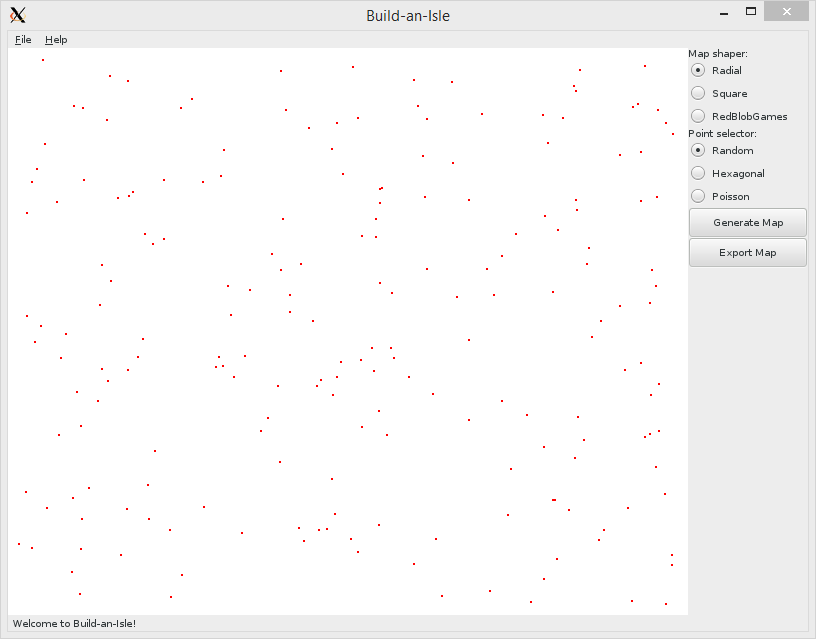
\includegraphics[width=0.8\linewidth]{points}
	\caption{Selecting points}
	\label{fig:algo:points}
\end{figure}

\begin{figure}
	\centering
	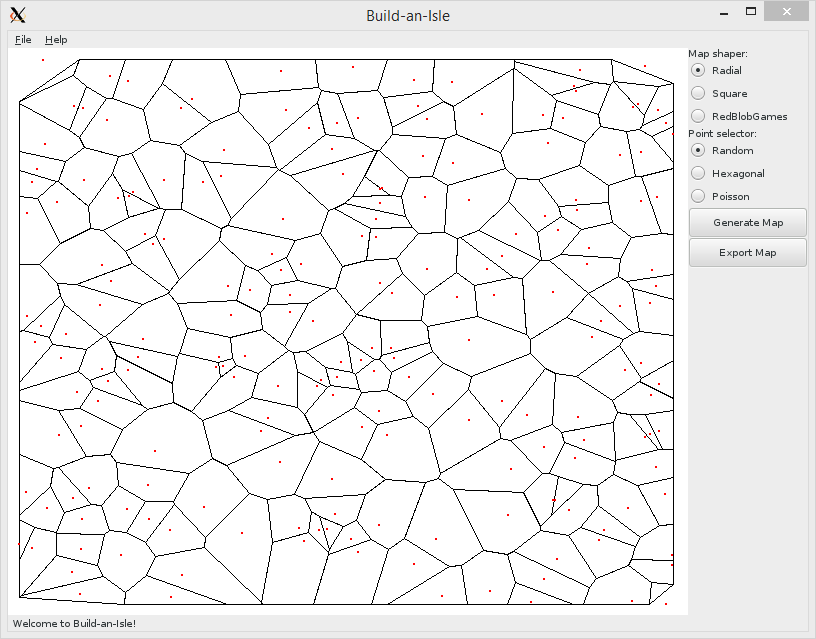
\includegraphics[width=0.8\linewidth]{voronoi}
	\caption{Building a Voronoi diagram}
	\label{fig:algo:voronoi}
\end{figure}

\begin{figure}
	\centering
	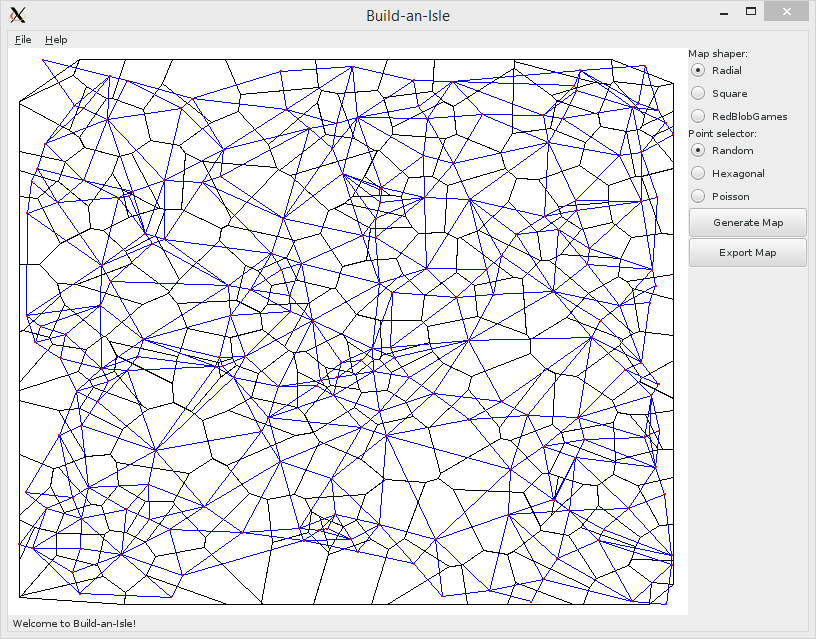
\includegraphics[width=0.8\linewidth]{delaunay}
	\caption{Delaunay triangulation}
	\label{fig:algo:delaunay}
\end{figure}

\begin{figure}
	\centering
	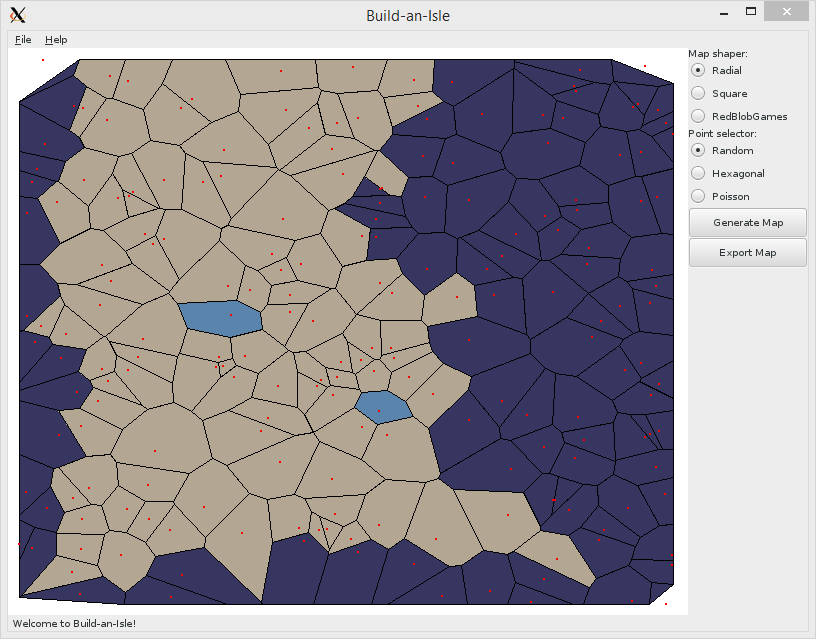
\includegraphics[width=0.8\linewidth]{polygons}
	\caption{Determining island shape}
	\label{fig:algo:polygons}
\end{figure}

\begin{figure}
	\centering
	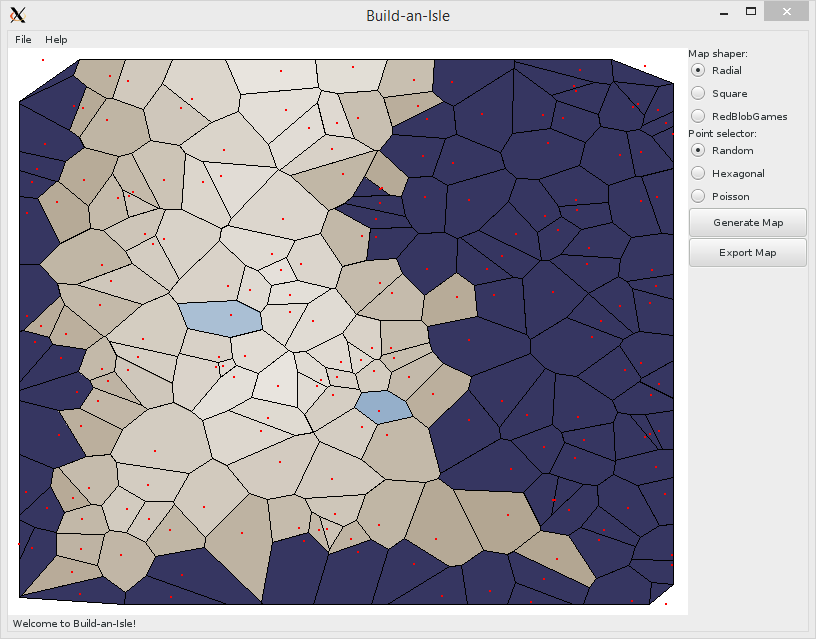
\includegraphics[width=0.8\linewidth]{elevation}
	\caption{Setting elevation}
	\label{fig:algo:elevation}
\end{figure}

%TODO: Similar images for the next steps

\subsection{Geometry generation}

The geometry of the map is generated preceding the visualisation phase. The maps are exported from the generator with all additional information intact to ensure their usefulness in all applications.

The surface of the islands can be generated rather straight-forward. For each center in the map data we generate as many triangles as there are borders associated with that center. Each of these triangles are formed with the center as the first vertex and the associated border's corners as the other two vertices.

\paragraph{Normal assignment}

If we simply use normals that are actually perpendicular to these triangles, the visualised terrain will look very harsh. Each face will be obviously individually distinguishable. This can be solved by assigning the same normal vector to vertices that share the same position. 
Our normal buffers can be constructed using a set of vertices and the normals will be calculated. Depending on whether or not smoothing is set to true or false normal vectors will be modified and set to the average x, y and z values of all normal vectors associated with vertices sharing the same position vector.

This 'smoothing' process takes an exponential amount of time when the number of input vectors is increased. Passing all generated triangles as one object resulted in this smooth normal calculation taking a very large amount of time when generating geometry for maps of significant size.

Fortunately we know that only a subset of generated vertices can share positions due to the fact that we know which centers are adjacent to eachother. Therefor we kept the vertices in seperate vertex buffers. In addition, we created an additional method to construct normals for a set of vertices while considering the set of vertices and associated normals that might affect what the smoothed normal values should be. This set consists of the vertices that are generated from the adjacent centers. 

\paragraph{River geometry}

To acquire more interesting geometry for our generated maps we decided to attempt to give the randomly assigned rivers a three-dimensional representation. We considered two main approaches, each with their individual challenges. Both methods basicly lower the geometric representation for any border that is part of a river and subsequently calculate a representation of the river bed depending on the river width at that point. This varying width showcases the underlying realistic representation of rivers very nicely. Simultaniously, it is the root of all problems concerning generation of a three-dimensional representation.

First off, it seemed logical to simply run through the centers as we had done previously, check which borders are part of a river and provide half of the river bed geometry based on that information. This would be the most elegant solution but it posed some problems in that there is no information on the river further up- or downstream. Figure ~\ref{riverproblem1} shows an instance where this method can run into trouble connecting river sections.

A solution to this problem and our second approach was to construct a tree of corners as nodes and river borders as edges for each of the existing rivers. Then we can start at the mouth of the river and work our way up. This way we have all the information we need to properly connect river sections of varying widths. Sadly this approach posed a new problem ~\ref{riverproblem2} which we did not previously experience due to the fact that we were processing each junction of river sections seperately. To solve this we needed elements from our first approach. 

Both approaches run into trouble ~\ref{riverproblem3} when the generated terrain contains very small cells and/or small borders. Irregular terrain can also result in the intersections of the river banks (parallels to the river edges) being very unpredictable, in our case this lead to a very spiky representation of the rivers in larger maps where there were bound to be some irregularities. The most reasonable solution to this problem was to guarantee more regular maps.

\begin{figure}
	\centering
	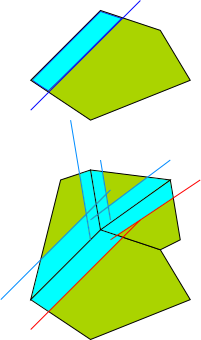
\includegraphics[width=0.8\linewidth]{mismatchedriverwidth}
	\caption{When we do not consider connecting river sections the generated geometry may not connect properly}
	\label{riverproblem1}
\end{figure}

\begin{figure}
	\centering
	
\includegraphics[width=0.8\linewidth]{obsoleteintersections}
	\caption{Some small borders may need to be disregarded when deciding where the river banks should connect, this can not be done on a junction to junction basis}
	\label{riverproblem2}
\end{figure}

\begin{figure}
	\centering
	
\includegraphics[width=0.8\linewidth]{outofpolygonintersections}
	\caption{Considering the possibility that the width of the river could cover an entire polygon makes the problem infinitely more complex}
	\label{riverproblem3}
\end{figure}

\subsection{System design}

Using wxWidgets we set up a window with the necessary controls to modify parameters with which to generate maps and export them. Within this window we will be using OpenGL to visualize the generation process and provide the user with an idea of what the map might look like in the viewer application.

\subsubsection{Preview rendering}

We want to give the user a good idea of what is being generated and how this is being done. This will highlight the workings of the generation process and allow the user to intuitively judge wether he or she should adjust the parameters.

\paragraph{Shaders}

Whenever we will be rendering anything we will be using appropriate shaders. For now we will be using a pair of relatively simple vertex and fragment shaders to be extended where needed. To start with they take into account the projection, position of the camera and model matrix for whichever object is being drawn. Furthermore each vertex has an associated position, normal and color. These are more or less minimal requirements to render anything. They also consider a single light source to add some dynamics to the map preview. 

Even with these simple shaders we can observe the effect of the calculations of the fragment shader in that eventual lighting dependent output colours are determined not per vertex but per pixel. This is one of the more obvious advantages of using our custom shaders.

The vertex shader simply takes the attributes such as position, normal and color or uv coordinate, determines the position on screen and interpolates the attributes for each pixel in between the vertices. The fragment shader is where things get interesting. Below~\ref{alg:point} is an example of our initial shader configuration. Some of the constants used should be implemented as uniforms to be adjustable per object to be drawn.
 
\begin{algo*}
\begin{sourcecode}
\textit{//Light properties}
LightPosition = vec3(50,50,10)
LightColor = vec3(1,0.8f,0.8f)
LightPower = 1500.0f
 
\algorithm{fragment($fPosition, fNormal, fColor, eyeVector, lightVector, normalVector$)}
\textit{//Material properties}
DiffuseColor = color
AmbientColor = 0.1f * color
SpecularColor = vec3(0.3,0.3,0.3)
\vspace{0.2cm}
\textit{//Angle between light and face}
n = normalize($normalVector$)
l = normalize($lightVector$)
cosTheta = clamp( dot( $n, l$ )$, 0, 1 $ )
\vspace{0.2cm}
\textit{//Angle between viewer and reflected light}
E = normalize($eyeVector$);
R = reflect($-l,n$);
cosAlpha = clamp( dot( $E,R$ )$, 0, 1$ );
\vspace{0.2cm}
\textit{//Final color determined taking all factors into account}
d = length( $lightPosition - fPosition$ )
brightness = LightPower / d$^2$
\return brightness * (AmbientColor + DiffuseColor * cosTheta + SpecularColor * cosAlpha)
\vspace{0.2cm}
\qend
\end{sourcecode}
        \caption{The fragment shader's method to return the final color}
        \label{alg:frag}
\end{algo*}

\subsection{Input/output}

Since we have a separate generator and viewer, we want the generator to be able to export maps to the disk and the viewer to be able to import.

To do this, we convert the Center, Corner and Edge objects to simple \texttt{struct}s, replacing pointers with indices.
Then, we store all relationships between centers, corner and edges to pairs of indices.
We store these structs in arrays, and write them directly to the disk.

When importing, we read from the disk into these arrays and use the indices to recreate the Center, Corner and Edge objects.

	
	\section{Design decisions}
	\label{sec:choices}
	%motivation of choices made

\subsection{Map file format}
When exporting our maps from the generator, all data remains intact. When importing the data structures that were present after generation are all restored. Alternatively we could have either put the data in a more commonly used format or we could have generated the geometry and merely exported that as an object file. The first alternative would in our case have unnecessarily complicated serialisation and deserialisation. The second alternative would have meant discarding much of the additional information concerning biomes and other intermediate data which could be interesting when the generated data is used in interactive applications.

\subsection{Terrain visualisation}
Within the limited time frame we chose to give rivers a geometric representation and focus on that instead of using texturing to indicate water. This posed interesting and tangible problems for us to solve while simultaniously turning out to be very challenging. Texturing the terrain appropriately posed other problems as the irregular polygon assignments made it very difficult to have the textures look seamless. Therefor the project does contain some code dealing with texturing but we decided to simply use biome appropriate coloring.

\subsection{Libraries}
We made both a map generation and viewing program and have used several libraries to provide the framework for our project.

\subsubsection{wxWidgets}
To provide the required functionality in the map generator specifically we decided to use the wxWidgets toolkit. This allows us to work towards a cross-platform solution and provides an easy way of implementing the necessary graphical user interface. To minimize the number of libraries are required to build both of the programs we intend to develop, we will also use wxWidgets to handle window setup for the map viewer. Even though it does not require most of the functionality provided by the library.

\subsubsection{OpenGL 4}
We wanted to make an effort to work with one of the most recent version of OpenGL. Partly because we were allready intending to write our own shaders to be able to have some more control over the eventual look of the generated landscape. The newer versions also provide some interesting types of shaders which may or may not be useful. Geometry and Tesselation shaders can actually alter the provided vertices which is interesting, but the downside is that we are trying to generate our maps before use instead of right before they are being shown to the user.

\subsubsection{Glew}
The wxGLCanvas provided by wxWidgets alone is not enough to be able to use our custom shaders. We will be using glew to take care of shader compilation and set up other advanced OpenGL features.
	
	\section{Discussion}
	\label{sec:discussion}
	While implementing the software, we have mostly stayed close to the algorithms described by Patel in \cite{redblob}.

The most important difference between our implementation and the demo implementation as given by Patel is that we have split up generation and visualisation.
This allows us to have a graphics-light generation application that is focused solely on enabling the user to tweak parameters and come up with a good terrain, while having a more immersive visualisation environment where a user can explore the terrain in more detail.

	
	\section{Results}
	\label{sec:results}
	%results & evaluation, explicitly mentioning of known limitations

	
	\section{Conclusion}
	\label{sec:conclusion}
	%conclusion and future work

In conclusion, we have implemented the basic terrain generation algorithm and an application that can import and visualise the generated terrain.

Since the visualiser has less features than originally planned, that is the main focus for future work.
The next steps for the visualiser are better interactivity (including walking, flying, generally moving around) and making the biomes look nicer.
While biomes are already assigned by the generator, they are currently shown by a single plain color, while adding a texture would already make them look much better.
A possible next step for biomes is adding vegetation and wildlife.


	\begin{appendices}
	\section{Map data structures}
	\label{appendix:mapdatastructures}
	\paragraph{Center} has the following properties:

\begin{itemize}
	\item Vec2 point
	\item bool water
	\item bool ocean
	\item bool coast
	\item bool border
	\item float elevation
	\item float moisture
	\item Biome biome
	\item Center[] neighbours
	\item Edge[] borders
	\item Corner[] corners
\end{itemize}

\paragraph{Corner} has the following properties:

\begin{itemize}
	\item Vec2 point
	\item bool water
	\item bool ocean
	\item bool coast
	\item bool border
	\item float elevation
	\item float moisture
	\item int river
	\item int watershed\_size
	\item Corner downslope
	\item Corner watershed
	\item Center[] touches
	\item Edge[] protrudes
	\item Corner[] adjacent
\end{itemize}

\paragraph{Edge} has the following properties:

\begin{itemize}
	\item Center delaunay0
	\item Center delaunay1
	\item Corner voronoi0
	\item Corner voronoi1
	\item int river
	\item Vec2 midway\_point
\end{itemize}


	\section{System design}
	\label{appendix:system}
	Using wxWidgets we set up a window with the necessary controls to modify parameters with which to generate maps and export them. Within this window we will be using OpenGL to visualize the generation process and provide the user with an idea of what the map might look like in the viewer application.

\subsection{Preview rendering}

We want to give the user a good idea of what is being generated and how this is being done. This will highlight the workings of the generation process and allow the user to intuitively judge wether he or she should adjust the parameters.

\paragraph{Shaders}

Whenever we will be rendering anything we will be using appropriate shaders. For now we will be using a pair of relatively simple vertex and fragment shaders to be extended where needed. To start with they take into account the projection, position of the camera and model matrix for whichever object is being drawn. Furthermore each vertex has an associated position, normal and color. These are more or less minimal requirements to render anything. They also consider a single light source to add some dynamics to the map preview.

Even with these simple shaders we can observe the effect of the calculations of the fragment shader in that eventual lighting dependent output colours are determined not per vertex but per pixel. This is one of the more obvious advantages of using our custom shaders.

The vertex shader simply takes the attributes such as position, normal and color or uv coordinate, determines the position on screen and interpolates the attributes for each pixel in between the vertices. The fragment shader is where things get interesting. Below~\ref{alg:point} is an example of our initial shader configuration. Some of the constants used should be implemented as uniforms to be adjustable per object to be drawn.

\begin{algo*}
\begin{sourcecode}
\textit{//Light properties}
LightPosition = vec3(50,50,10)
LightColor = vec3(1,0.8f,0.8f)
LightPower = 1500.0f

\algorithm{fragment($fPosition, fNormal, fColor, eyeVector, lightVector, normalVector$)}
\textit{//Material properties}
DiffuseColor = color
AmbientColor = 0.1f * color
SpecularColor = vec3(0.3,0.3,0.3)
\vspace{0.2cm}
\textit{//Angle between light and face}
n = normalize($normalVector$)
l = normalize($lightVector$)
cosTheta = clamp( dot( $n, l$ )$, 0, 1 $ )
\vspace{0.2cm}
\textit{//Angle between viewer and reflected light}
E = normalize($eyeVector$);
R = reflect($-l,n$);
cosAlpha = clamp( dot( $E,R$ )$, 0, 1$ );
\vspace{0.2cm}
\textit{//Final color determined taking all factors into account}
d = length( $lightPosition - fPosition$ )
brightness = LightPower / d$^2$
\return brightness * (AmbientColor + DiffuseColor * cosTheta + SpecularColor * cosAlpha)
\vspace{0.2cm}
\qend
\end{sourcecode}
        \caption{The fragment shader's method to return the final color}
        \label{alg:frag}
\end{algo*}

	\end {appendices}

	\bibliographystyle{plain}
	\bibliography{bibliography}
\end{document}
